\chapter{Hales-Jewett theorem}

We will now jump to another topic and mainly the Hales-Jewett theorem. This was actually motivated by famous Van der Waerden theorem \ref{van-der-waerden}.

\begin{thm}
	For every $n > 0$ and every finite coloring of integers there exists monochromatic arithmetic progression of length $n$, i.e. $a, a + b, a + 2b, \dots, a + (n-1)b$ for $b > 0$.
	\label{van-der-waerden}
\end{thm}

But the main issue is that this theorem is rather more algebraic and also used in combinatorics. For example we could create an auxiliary hypergraph $H = (\N, \text{all pregressions of length }n)$ so that we are looking at edges.

\begin{topic}{Multidimensional Tic-Tac-Toe}
	Lets consider $\Sigma$ finite alphabet (set). Then $\Sigma^n$ is set of functions $[n] \to \Sigma$ (usually called words). Lets define a hypergraph by the following set. $L \subseteq \Sigma^n$ is combinatorial line if $M \subseteq \{1, 2, \dots, n\}$ nonempty and $f: [n] \to \Sigma$ such that
	
	$$
	L = \left\{g | \exists c \in \Sigma \ g(i) = \left\{
	\begin{array}{ll}
		c & \text{if } i \in M \\
		f(i) & \text{if } i \notin M
	\end{array}
	\right.\right\}.
	$$
	
	\begin{example}
		Lets have $w = (\{\lambda\} \cup \Sigma)^n$ then lets have $A\lambda\lambda B$ which can either be $AAAB$ or $ABBB$. So formally $M = \{2,3\}$ and $f = AAAB$.
	\end{example}

	\begin{figure}[!ht]\centering
		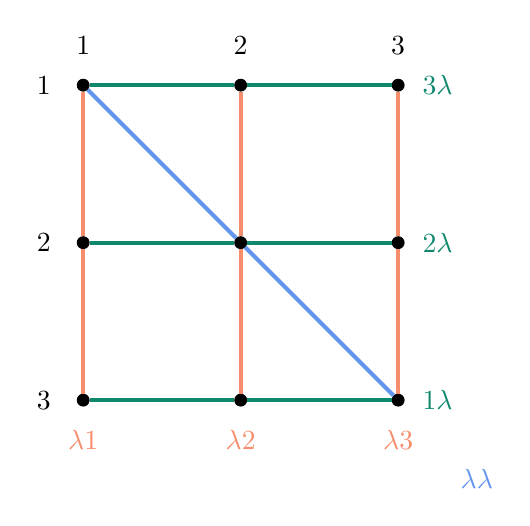
\begin{tikzpicture}[n/.style = {draw, circle, fill, inner sep=1.5pt},
			l/.style = {line width=1.5pt},
			o/.style = {Melon},
			g/.style = {PineGreen},
			b/.style = {CornflowerBlue}]
			\foreach \j in {1,...,3} {
				\foreach \i in {1,...,3} {
					\node[n] (\j-\i) at (2*\j,2*\i) {};
				}
			}
			\foreach \j in {1,...,3}{
				\node (l1-\j) at (1.5, 8 - 2*\j) {\j};
			}
			\foreach \j in {1,...,3}{
				\node (l2-\j) at (2*\j, 6.5) {\j};
			}
			\foreach \j in {1,...,3}{
				\draw[o,l] (\j-1) to (\j-2) to (\j-3);
				\node[o] at (2*\j, 1.5) {$\lambda$\j};
				\draw[g,l] (1-\j) to (2-\j) to (3-\j);
				\node[g] at (6.5, 2*\j) {\j$\lambda$};
			}
			\draw[b,l] (1-3) to (2-2) to (3-1);
			\node[b] at (7,1) {$\lambda\lambda$};	
		\end{tikzpicture}
		\caption{Combinatorial representation of combinatorial lines for $\Sigma = \{1,2,3\}$ and $n =2$. Which we can see we obtain a hypergraph $H = (\Sigma^n, \text{Lines})$.}
	\end{figure}
\end{topic}

\begin{thm}{Hales-Jewett, 1963}
	For every finite $\Sigma$ and finite $n > 0$ $\exists N > 0$ such that the chromatic number of $H(\Sigma^n, \text{Lines})$ is at least $n$.
\end{thm}